\section*{Opgave 2}\addcontentsline{toc}{section}{Opgave 2}\refstepcounter{section}
Overfladen $\mathcal{S}$ er givet som grafen for funktionen
\begin{equation}
	f(x,y)=e^{x^2-2x+4y^2-3}
\label{eq:opg2}
\end{equation}

\subsection*{a)}\addcontentsline{toc}{subsection}{a)}\refstepcounter{subsection}
En ligning for tangentplanet til overfladen $\mathcal{S}$ �nskes fundet i punktet $\big(1,-1,f(1,-1)\big)$

Generelt er ligningen for et tangentplan til et plan $z=f(x,y)$ gennem punktet $\big(a,b,f(a,b)\big)$ givet\footcite[685, 722]{adamsessex} ved \eqref{eq:_opg2_tangentplan}
\begin{equation}
	\boxed{
	z = f(a,b) + f_1(a,b)(x-a) + f_2(a,b)(y-b)
	}
\label{eq:_opg2_tangentplan}
\end{equation}
hvor
\begin{align*}
	f_1(a,b) = \Big(\frac{\partial}{\partial x}f(x,y)\Big)\Big|_{(a,b)}\\
	f_2(a,b) = \Big(\frac{\partial}{\partial y}f(x,y)\Big)\Big|_{(a,b)}
\end{align*}

F�rst findes $f(x,y)$ partielt differentieret med respekt til $x$, evalueret ved $(1,-1)$
\begin{align*}
	& \frac{\partial}{\partial x} \left( e^{x^2-2x+4y^2-3} \right)\Big|_{(1,-1)}\\
	&= e^{x^2-2x+4y^2-3}(2x-2)\big|_{(1,-1)}\\
	&= e^{1^2-2+4(-1)^2-3}(2-2)\\
	&= 0
\end{align*}

og derefter $f(x,y)$ partielt differentieret med respekt til $y$, evalueret ved $(1,-1)$
\begin{align*}
	& \frac{\partial}{\partial y} \left( e^{x^2-2x+4y^2-3} \right)\Big|_{(1,-1)}\\
	&= e^{x^2-2x+4y^2-3}(8y)\big|_{(1,-1)}\\
	&= e^{1^2-2+4(-1)^2-3}(-8)\\
	&=-8
\end{align*}

Nu haves det, der skal til for at bestemme tangentplanet - se ligning \eqref{eq:_opg2_tangentplan} - til $f(x,y)$
\begin{align*}
	z &= f(a,b) + f_1(a,b)(x-a) + f_2(a,b)(y-b)\\
	&= e^{1^2-2+4(-1)^2-3} + (-8)(y-(-1))\\
	&= -8y-7
\end{align*}
Planet, der her er fundet, har en $z$-v�rdi der kun er afh�ngig af $y$, og m� derfor v�re parallelt med $x$-aksen.

%%%%%%%%%%%%%
\subsection*{b)}\addcontentsline{toc}{subsection}{b)}\refstepcounter{subsection}
For at bestemme niveaukurver til funktionen $f(x,y)=e^{x^2-2x+4y^2-3}$ lader vi $f(x,y)$ antage en konstant v�rdi $K$. Vi har at g�re med en ellipseform; $-2x$ leddet g�r, at formen ikke l�ngere har centrum i $(0,0)$ og, som vi skal se, afviger excentriciteten ogs� fra $0$ (s� det ikke er en cirkel). Dvs
\begin{align*}
	K &= e^{x^2-2x+4y^2-3}\iff\\
	\ln K &= x^2-2x+4y^2-3\iff\\
	\ln K &= (x-1)^2+4y^2-4\iff\\
	\dfrac{\ln K + 4}{4} &= \dfrac{(x-1)^2}{4}+y^2\iff\\
	1 &= \dfrac{(x-1)^2}{\ln K + 4}+\dfrac{y^2}{\frac{1}{4}\ln K + 1}
\end{align*}

Vi har alts� at g�re med en ellipse med centrum i $(1,0)$ og storakse $a$ og lilleakse $b$ givet som
\begin{align*}
	a &= \sqrt{\ln K + 4}\\
	b &= \sqrt{\frac{1}{4}\ln K + 1}
\end{align*}

For at skitsere niveaukurver ser vi, som eksempel, f�rst p� det tilf�lde hvor $K=e$
\begin{align*}
	K &= e \implies\\
	1 &= \dfrac{(x-1)^2}{5}+\dfrac{y^2}{\nicefrac{5}{4}}
\end{align*}

\begin{figure}[htb]
	\begin{center}
	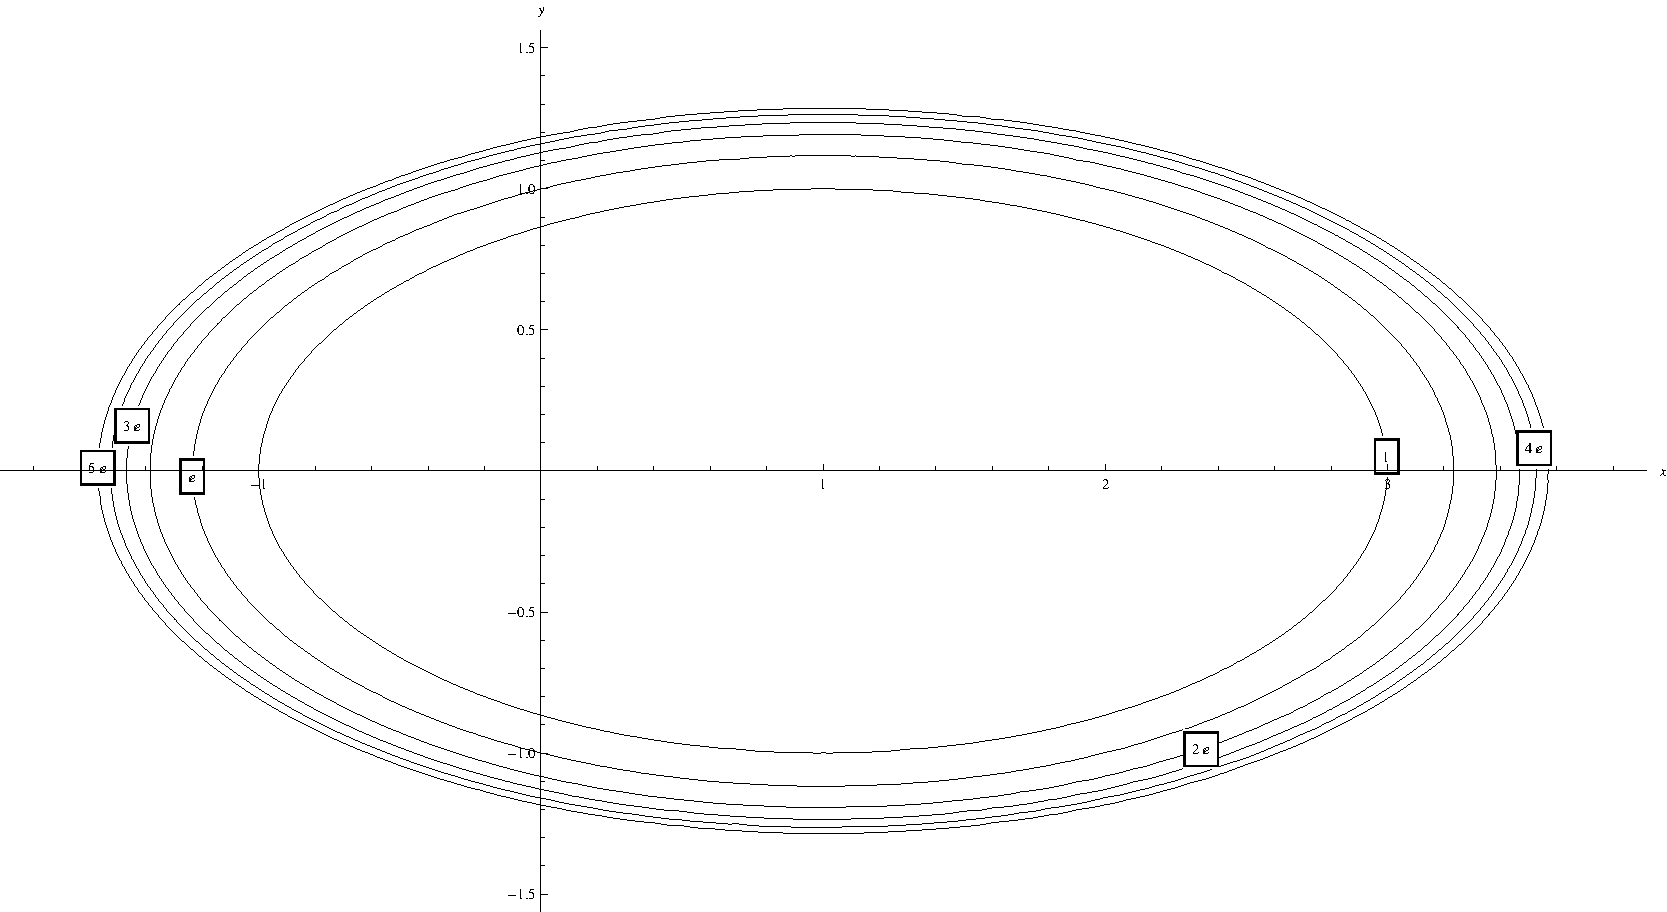
\includegraphics[width=\textwidth]{opg2_nivkurver.pdf} %trim=l b r t
	\caption{Niveaukurver}
	\label{fig:opg2_nivkurver}
	\end{center}
\end{figure}

Sk�ringer med $x$-aksen er 
\begin{align*}
	1 &= \dfrac{(x-1)^2}{5}\iff\\
	x &= \pm\sqrt{5}+1\implies\\
	x &\approx -1.24 \vee x \approx 3.24
\end{align*}
og sk�ringer med $y$-aksen er
\begin{align*}
	1 &= \dfrac{1}{5}+\dfrac{y^2}{\nicefrac{5}{4}}\iff\\
	y &= \pm 1
\end{align*}
Stor- og lilleaksernes l�ngde er
\begin{align*}
	a &= \sqrt{5} \approx 2,24\\
	b &= \sqrt{\frac{5}{4}} \approx 1,12
\end{align*}

P� figur \ref{fig:opg2_nivkurver} ses niveaukurver (hvor $K = 1, e, 2e, 3e, 4e, 5e$) afbilledet vha. \textit{Mathematica}